\documentclass[12pt,a4paper]{ctexart}
\usepackage[a4paper,margin=2.3cm]{geometry}
\usepackage{amsmath,amssymb}
\usepackage{booktabs}
\usepackage{graphicx}
\usepackage{float}
\usepackage{caption}
\usepackage{hyperref}
\hypersetup{colorlinks=true,linkcolor=blue,urlcolor=blue,citecolor=blue}

\title{PRCV 第二次作业报告\\霍夫变换与角点检测}
\author{姓名：许政阳 \quad 学号：231880081}
\date{\today}

\begin{document}
\maketitle
\tableofcontents
\newpage

\section{作业概述}
本报告完成了题目要求的三部分内容：
\begin{itemize}
    \item 理论问题（Q2.1, Q2.3）的完整推导；
    \item 代码实现（Q3.3, Q3.4, Q3.5）及关键算法说明；
    \item 在全部 10 张图像上的实验结果和讨论（Q4.1, Q4.2）。
\end{itemize}

实现脚本均放在 \texttt{python/} 目录下，并且所有图像读写均采用相对路径。最终提交中包含：
\begin{itemize}
    \item \texttt{python/houghScript.py}
    \item \texttt{python/myHoughTransform.py}
    \item \texttt{python/myHoughLines.py}
    \item \texttt{python/harris\_cornerScript.py}
\end{itemize}

\section{理论问题}
\subsection{Q2.1 卷积交换律证明}
已知连续函数卷积定义为
\begin{equation}
(f * g)(x) = \int_{-\infty}^{+\infty} f(y)g(x-y)\,dy.
\end{equation}
令
\[
u = x - y \Rightarrow y = x-u,\quad dy = -du.
\]
当 $y$ 从 $-\infty$ 到 $+\infty$ 时，$u$ 从 $+\infty$ 到 $-\infty$。代入并调整积分上下限可得
\begin{align}
(f * g)(x)
&= \int_{+\infty}^{-\infty} f(x-u)g(u)(-du) \\
&= \int_{-\infty}^{+\infty} g(u)f(x-u)\,du \\
&= (g * f)(x).
\end{align}
因此卷积满足交换律：
\[
f*g = g*f.
\]

\subsection{Q2.3 霍夫变换直线参数化}
\subsubsection*{(1) 点在霍夫空间对应正弦曲线}
霍夫直线参数化为
\begin{equation}
\rho = x\cos\theta + y\sin\theta.
\end{equation}
令
\[
r=\sqrt{x^2+y^2},\quad \phi=\mathrm{atan2}(y,x),
\]
则
\[
x=r\cos\phi,\quad y=r\sin\phi.
\]
代入上式得
\begin{align}
\rho &= r\cos\phi\cos\theta + r\sin\phi\sin\theta \\
&= r\cos(\theta-\phi).
\end{align}
故在 $(\rho,\theta)$ 空间里，图像中每个点对应一条余弦曲线，其\textbf{振幅}为
\[
A=r=\sqrt{x^2+y^2},
\]
\textbf{相位}为
\[
\phi=\mathrm{atan2}(y,x).
\]

\subsubsection*{(2) 为什么用 $(\rho,\theta)$ 而不是 $(m,c)$}
\begin{itemize}
    \item 斜率截距形式 $y=mx+c$ 在垂直线处 $m\to\infty$，参数会发散；
    \item $(\rho,\theta)$ 对任意方向直线都稳定，参数域有界，便于离散投票；
    \item 霍夫累加器中每个单元对应唯一几何意义（某组法向参数）。
\end{itemize}

两种形式关系如下。由
\[
\rho = x\cos\theta + y\sin\theta
\]
得
\[
y = -\frac{\cos\theta}{\sin\theta}x + \frac{\rho}{\sin\theta},\quad (\sin\theta\neq 0),
\]
故
\[
m=-\frac{\cos\theta}{\sin\theta},\quad c=\frac{\rho}{\sin\theta}.
\]
当 $\sin\theta=0$ 时对应垂直线，方程为 $x=\rho$。

\subsubsection*{(3) $\rho,\theta$ 的取值范围}
设图像点满足 $x\in[1,W], y\in[1,H]$。根据柯西不等式，
\[
|\rho| = |x\cos\theta+y\sin\theta|
\le \sqrt{x^2+y^2}\sqrt{\cos^2\theta+\sin^2\theta}
\le \sqrt{W^2+H^2}.
\]
因此
\[
|\rho|_{\max}=\sqrt{W^2+H^2}.
\]
若实现中按题面要求只保留非负 $\rho$，则可设
\[
\rho\in[0,\sqrt{W^2+H^2}],\quad \theta\in[0,2\pi].
\]

\subsubsection*{(4) 三个点的霍夫曲线与交点}
对点 $(10,10),(20,20),(30,30)$，它们在原图中共线于 $y=x$，对应直线参数在霍夫空间有公共交点。绘图结果如图 \ref{fig:q23} 所示。

\begin{figure}[H]
    \centering
    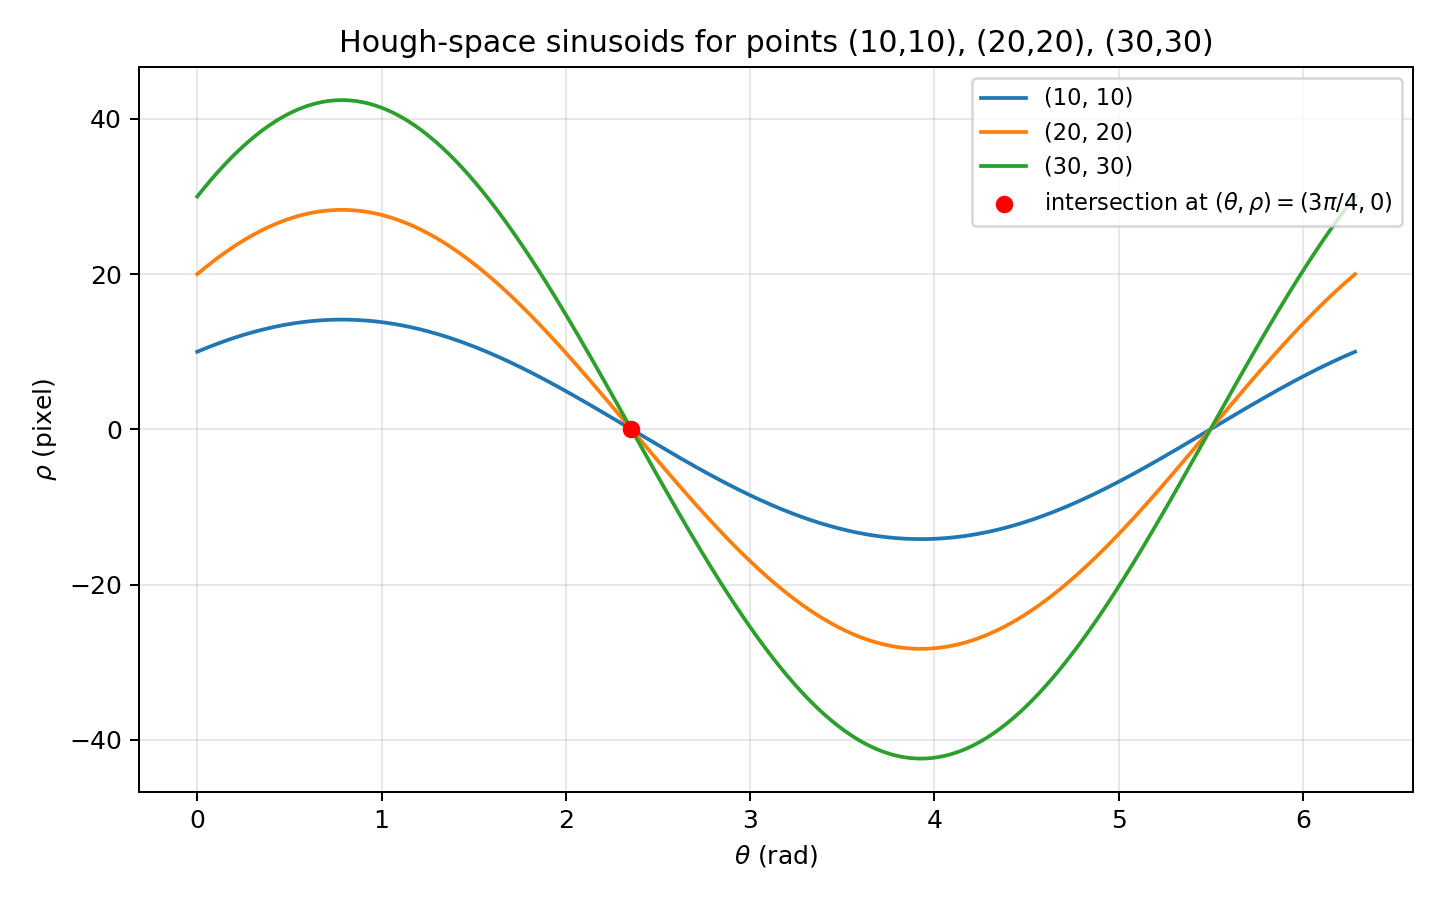
\includegraphics[width=0.78\textwidth]{results/q23_hough_sinusoids.png}
    \caption{Q2.3：三个点在霍夫空间对应曲线及交点}
    \label{fig:q23}
\end{figure}

三点所在直线为
\[
y=x \Rightarrow m=1,\ c=0.
\]
这也与霍夫曲线交点所代表的同一直线一致。

\section{代码实现}
\subsection{Q3.3 霍夫变换 \texttt{myHoughTransform}}
我实现了函数：
\[
[\texttt{img\_hough},\ \texttt{rhoScale},\ \texttt{thetaScale}] =
\texttt{myHoughTransform(img\_threshold,\ rhoRes,\ thetaRes)}.
\]
关键步骤如下：
\begin{enumerate}
    \item 设定参数域：$\theta\in[0,2\pi)$，$\rho\in[0,\sqrt{W^2+H^2}]$；
    \item 对阈值边缘图中每个非零像素点 $(x,y)$，按
    \[
    \rho = x\cos\theta + y\sin\theta
    \]
    计算离散 $\theta$ 下的所有 $\rho$；
    \item 丢弃负 $\rho$ 的投票，仅对合法单元累加；
    \item 输出霍夫累加器及尺度数组。
\end{enumerate}

图 \ref{fig:hough_acc} 给出了某张图像（\texttt{img01}）的 \texttt{img\_hough} 可视化结果。

\begin{figure}[H]
    \centering
    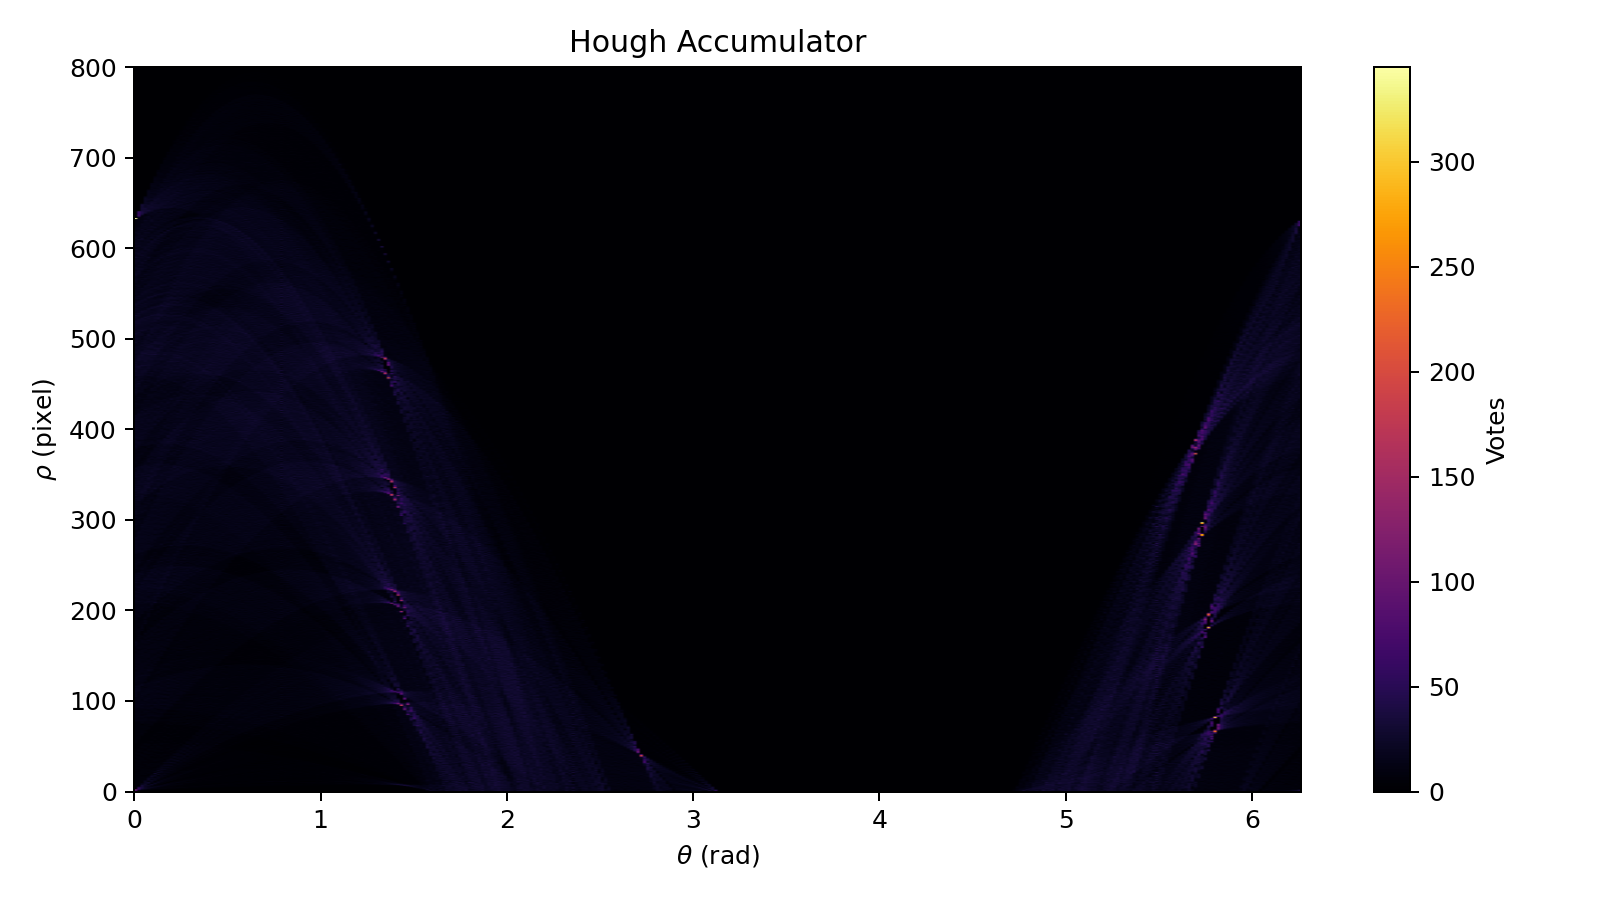
\includegraphics[width=0.8\textwidth]{results/img01_hough_accumulator.png}
    \caption{Q3.3：霍夫累加器示例（img01）}
    \label{fig:hough_acc}
\end{figure}

\subsection{Q3.4 直线提取 \texttt{myHoughLines}}
我实现了函数
\[
[\texttt{rhos},\ \texttt{thetas}] = \texttt{myHoughLines(img\_hough,\ nLines)}.
\]
流程如下：
\begin{enumerate}
    \item 对累加器做局部非极大值抑制（NMS），窗口大小为 $11\times 11$；
    \item 仅保留局部峰值单元；
    \item 按投票强度降序取前 \texttt{nLines} 个峰值，返回其行列坐标；
    \item 在 \texttt{houghScript.py} 中映射回 $(\rho,\theta)$ 并绘制红色直线。
\end{enumerate}

同时，脚本还叠加了 OpenCV \texttt{HoughLinesP} 的绿色线段用于对照（仅用于比较，不参与我的实现）。

\begin{figure}[H]
    \centering
    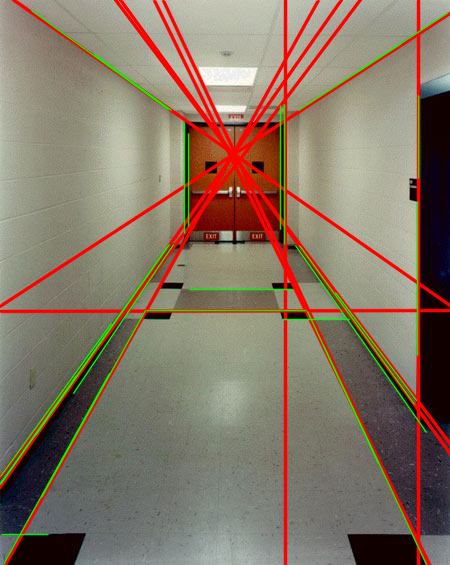
\includegraphics[width=0.78\textwidth]{results/img03_hough_lines.png}
    \caption{Q3.4：直线检测示例（红：本实现；绿：OpenCV 对照）}
    \label{fig:hough_one}
\end{figure}

\subsection{Q3.5 多尺度 Harris 角点检测}
在 \texttt{harris\_cornerScript.py} 中实现多尺度 Harris：
\begin{enumerate}
    \item 尺度集合：$\sigma\in\{1.0,1.6,2.2,3.0,4.0\}$；
    \item 在每个尺度下计算梯度 $I_x,I_y$，构造二阶矩阵分量
    \[
    S_{xx}=G_{\sigma_s}*(I_x^2),\quad
    S_{yy}=G_{\sigma_s}*(I_y^2),\quad
    S_{xy}=G_{\sigma_s}*(I_xI_y),
    \]
    其中 $\sigma_s=1.5\sigma$；
    \item 计算 Harris 响应
    \[
    R=\det(M)-k\cdot \mathrm{trace}(M)^2,\quad k=0.04;
    \]
    \item 在每个尺度做阈值与局部极大值筛选，再做跨尺度抑制；
    \item 将角点画成红色圆圈，半径与尺度成比例。
\end{enumerate}

\begin{figure}[H]
    \centering
    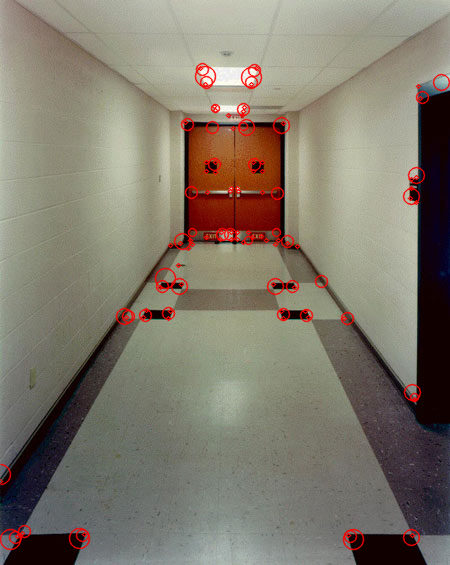
\includegraphics[width=0.78\textwidth]{results/img03_harris_multiscale.png}
    \caption{Q3.5：多尺度 Harris 角点示例（圆圈半径表示尺度）}
    \label{fig:harris_one}
\end{figure}

\section{实验讨论}
\subsection{Q4.1 霍夫变换讨论}
我在全部 10 张图像上运行了霍夫检测脚本，结果总览见图 \ref{fig:hough_all}。

\begin{figure}[H]
    \centering
    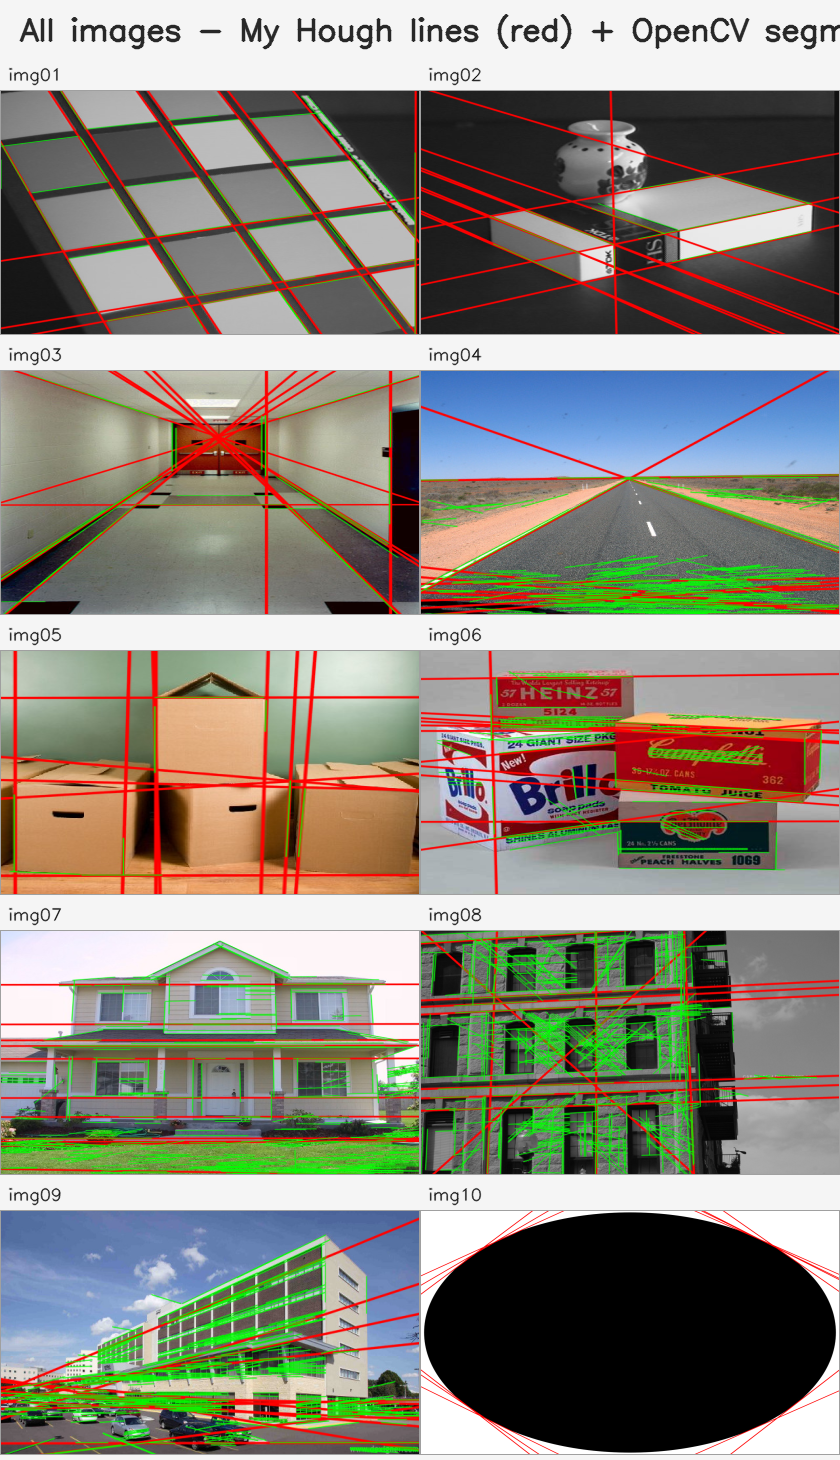
\includegraphics[width=\textwidth]{results/hough_all_grid.png}
    \caption{全部图像的霍夫直线检测结果总览}
    \label{fig:hough_all}
\end{figure}

统计结果如下（边缘像素数越多，通常需要更谨慎设置参数）：
\begin{table}[H]
    \centering
    \caption{霍夫与 Harris 统计量（全数据）}
    \begin{tabular}{cccccc}
        \toprule
        图像 & 边缘像素数 & 霍夫最大票数 & Harris 角点数 & OpenCV 线段数 \\
        \midrule
        img01 & 9030  & 345 & 158 & 65  \\
        img02 & 4577  & 183 & 131 & 10  \\
        img03 & 6468  & 219 & 129 & 26  \\
        img04 & 18216 & 231 & 72  & 172 \\
        img05 & 4259  & 109 & 85  & 9   \\
        img06 & 19440 & 204 & 250 & 106 \\
        img07 & 37110 & 410 & 250 & 314 \\
        img08 & 36468 & 285 & 250 & 372 \\
        img09 & 29616 & 545 & 250 & 300 \\
        img10 & 4531  & 89  & 250 & 0   \\
        \bottomrule
    \end{tabular}
\end{table}

\textbf{问题 1：同一套参数是否在所有图像都表现良好？}\\
不能。统一参数在结构规整、对比清晰的图像上效果较好，但在纹理复杂或边缘断裂严重的图像上，误检和漏检明显增多。

\textbf{问题 2：最佳参数如何随图像变化？}\\
\begin{itemize}
    \item 边缘较稀疏：可降低 Canny 阈值、增大 \texttt{nLines}；
    \item 纹理较密集：应提高 Canny 阈值、增大 NMS 窗口，避免重复峰值；
    \item 对精度要求高：减小 \texttt{thetaRes} 可提高角度精度，但计算更慢且易分票。
\end{itemize}

\textbf{问题 3：哪个步骤最容易引发问题？}\\
最敏感步骤是\textbf{边缘提取与峰值筛选}。边缘图质量直接决定投票质量，NMS 不足会导致同一条线被重复输出。

\textbf{问题 4：改进措施}\\
\begin{itemize}
    \item 引入自适应阈值或基于图像统计量自动设定 Canny 参数；
    \item 使用梯度方向约束投票角度区间，减少噪声投票；
    \item 在峰值提取阶段加入最小角度/距离间隔约束；
    \item 采用分层分辨率策略先粗后细定位 $(\rho,\theta)$。
\end{itemize}

\subsection{Q4.2 Harris 角点检测讨论}
我在全部图像上运行了多尺度 Harris，结果总览见图 \ref{fig:harris_all}。

\begin{figure}[H]
    \centering
    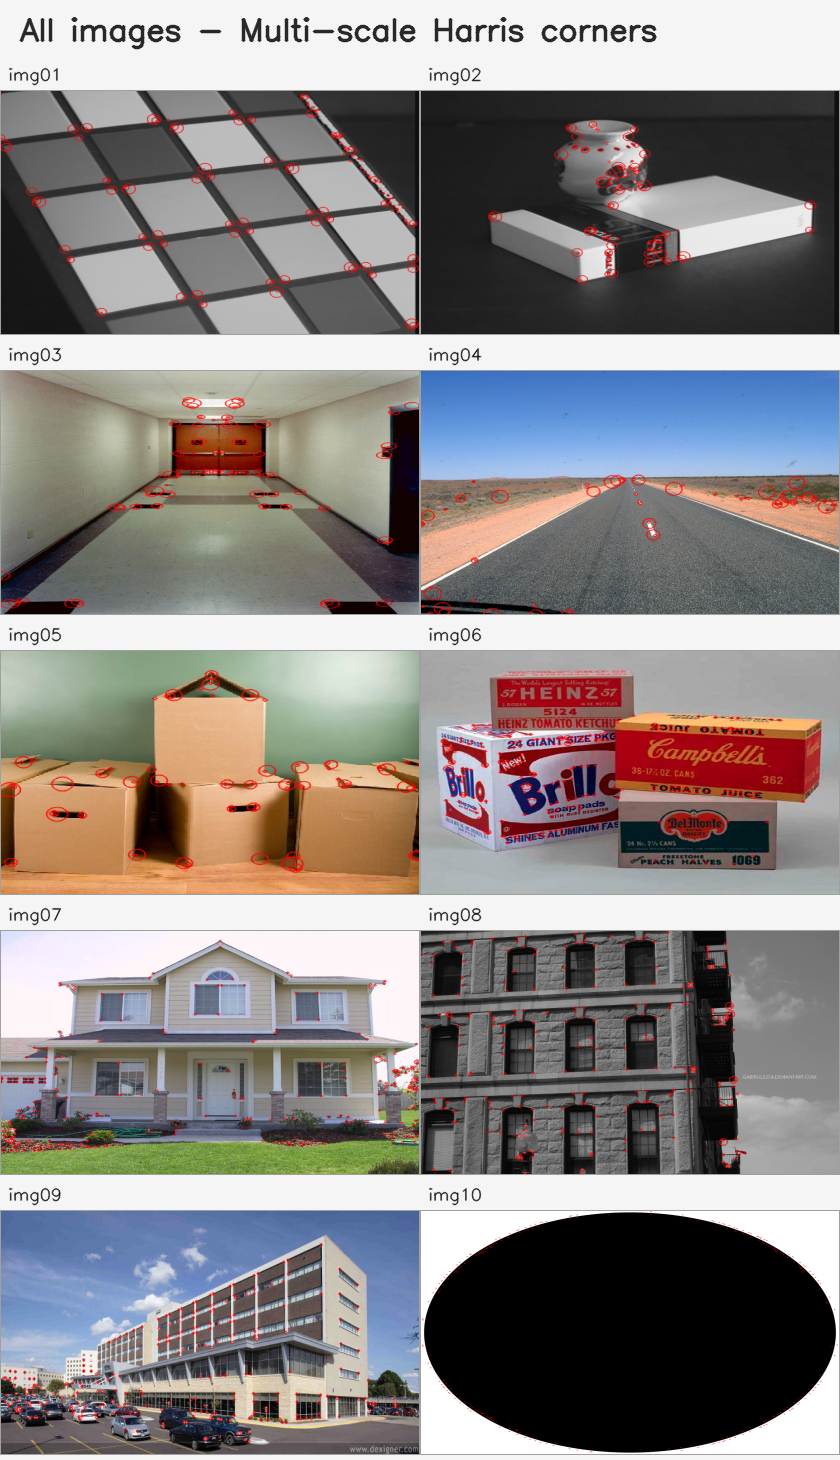
\includegraphics[width=\textwidth]{results/harris_all_grid.png}
    \caption{全部图像的多尺度 Harris 角点结果总览}
    \label{fig:harris_all}
\end{figure}

\textbf{问题 1：不同尺度角点特点}\\
\begin{itemize}
    \item 小尺度角点：数量更多，能捕捉细节，但对噪声敏感；
    \item 大尺度角点：数量较少，更稳定，更偏向显著结构（建筑拐角、强纹理交叉）；
    \item 多尺度融合能兼顾细节与稳定性，较单尺度更鲁棒。
\end{itemize}

\textbf{问题 2：好的角点应具备什么特征？}\\
好的角点应同时满足：
\begin{itemize}
    \item 在两个正交方向上都有较强灰度变化（非单向边缘）；
    \item 在尺度变化下位置稳定、响应较强；
    \item 重复性好（视角或光照变化后仍可检测）；
    \item 空间分布合理，不应全部集中在局部噪声区域。
\end{itemize}

\section{结论}
本次作业完整实现并验证了霍夫直线检测与多尺度 Harris 角点检测。实验表明：参数选择显著影响结果，统一参数难以覆盖所有图像；通过非极大值抑制、多尺度融合与合理阈值设计，可以显著提升检测稳定性。后续若进一步结合自适应参数与方向先验，检测性能还可继续提高。

\end{document}
